\begin{appendices}
%\chapterimage{icesymmetries.jpg}
%\chapter{Gauge symmetries}
%\label{ch:gauge}
%\textcolor{red}{NOG NIET GEDAAN}

%The difference between global and local symmetries are not straightforward for everybody. In this appendix I try to give a better view of the matter.

%Imagine that at each point in space and time there is a circle attached to it. If one shifts all circles of all points with a fixed angle the underlying physics hasn't changed. If we look at the whole in a different angle, nothing seems to be changed as everything holds the same relative orientation. This is a global symmetry. For local symmeries we instead shift each circle through a different angle, but an angle that changes smoothly from point to point and in a way that we can say how that angle is varying between different nearby regions. Then it will turn out that we can describe that rotation angle by means of a so-called gauge field, which just lets us transport the charged scalar field from one point in space time to another, taking account of how the rotation angle of the circle is changing. A gauge is a kind of coordinate system that is varying depending on the location with respect to some underlying space. In physics we are almost always concerned with space-time as the underlying space, and we are typically interested in theories that are invariant with respect to the choice of gauge or coordinate system. 

%Dan wat uitleg vanuit je QFT boek en de dingen hieronder:
%Je wilt je derivative anders doen werken in je theory onder een transformatie, maar daarvoor heb je een veld nodig. M.a.w.: dankzij een veld heb je lokale ijktransformatie mogelijk!


%Now consider if one wished to not only make global changes of phase but also local gauge transformations. Then the phase α would have to become a spatial function, α(x). Note now that the kinetic term would pick up derivatives of α(x), so the action is not automatically invariant under this change. In order to make it invariant and enforce such a symmetry, one must rewrite the transformation law so that there is a new type of derivative Dμϕ, which under the change of phase on ϕ transforms in the same fashion,
%Dμϕ→eiα(x)Dμϕ.
%This derivative is said to be a gauge covariant derivative, in that it varies in the fashion that the field does when a gauge transformation is performed. To construct such a derivative, one introduces a new field in space called the gauge field whose transformation law under the gauge transformation will be prescribed so as to give the above law. The gauge derivative then becomes
%Dμϕ=∂μϕ+igAμϕ.
%(Note that the gauge derivative acting on ϕ∗ has the opposite sign in front of i, from the complex conjugate of this equation). The gauge field is playing the role of a connection field. In order for the derivative to be gauge covariant, the gauge field must transform as
%Aμ→Aμ+1g∂μα. 

%\chapterimage{planck_crop.png}
%\chapter{Planck's law}
%\label{ch:planck}
%%bron: http://hyperphysics.phy-astr.gsu.edu/hbase/quantum/rayj.html
%\section{Electromagnetic waves in a cubical cavity}
%Suppose we have EM waves in a cavity at equilibrium with its surroundings. These waves must satisfy the wave equation in three dimensions:

%\begin{equation}
%\label{eq:wave}
%\frac{\partial^2 \Psi}{\partial x^2} + \frac{\partial^2 \Psi}{\partial y^2} + \frac{\partial^2 \Psi}{\partial z^2} = \frac{1}{c^2} \frac{\partial^2 \Psi}{\partial t^2}.
%\end{equation}
%The solution must give zero amplitude at the walls. A non-zero value would mean energy is dissipated through the walls which is in contradiction to our equilibrium assumption. A general solution takes the form of

%\begin{equation}
%\Psi(x,y,z,t) = \Psi_0 \sin{k_1x} \sin{k_2y} \sin{k_3z} \sin{k_4 t},
%\end{equation}
%which, after requiring $k_n L = n \pi$ with $n=0,1,2...$ and $k_4 \frac{\lambda}{2c} = \pi$, leads to

%\begin{equation}
%\Psi(x,y,z,t) = \Psi_0 \sin{\left(\frac{n_1 \pi x}{L}\right)} \sin{\left(\frac{n_2 \pi y}{L}\right)} \sin{\left(\frac{n_3 \pi z}{L}\right)} \sin{\left(\frac{2\pi ct}{\lambda}\right)}.
%\end{equation}

%From the wave equation it is easy to find that

%\begin{equation}
%\label{eq:n}
%n^2 = n_1^2 + n_2^2 + n_3^2 = \frac{4L^2}{\lambda^2},
%\end{equation}
%which span up a sphere in ``n-space'' with a volume of $\frac{1}{8}\frac{4}{3}\pi n^{3/2}$, where the first term originates from the positive nature of $n_{1,2,3}$. Because there are two possible polarizations of the waves one has to multiply with an additional factor 2. The number of modes per unit wavelength is equal to

%\begin{equation}
%\frac{dN}{d\lambda} \times \frac{1}{L^3} = \frac{d}{d\lambda}\left[\frac{8\pi L^3}{3\lambda^3}\right]  \times \frac{1}{L^3} = - \left[\frac{8\pi}{\lambda^4}\right].
%\end{equation}
%\subsection{Classical approach}
%Following the principle of equipartition of energy, each standing wave mode will have an average enkergy $kT$ with $k$ the Boltzmann constant and $T$ the temperature in Kelvin. The energy density is then:

%\begin{equation}
%\frac{du}{d\lambda} = -kT \frac{8\pi}{\lambda^4}.
%\end{equation}
%In function of frequency $\nu = \frac{c}{\lambda}$:

%\begin{equation}
%\label{eq:rayleigh}
%\frac{du}{d\nu} = -\frac{c}{\lambda^2} \frac{du}{d\lambda} = \frac{8\pi kT \nu^2}{c^3},
%\end{equation}
%also known as the Rayleigh-Jeans law\footnote{This is often quoted per unit of staradian, which results in $\frac{2 kT \nu^2}{c^3}$}. Problem: divergence

%\subsection{Quantum approach}
%The energy levels from a quantized harmonic oscillator are equal to

%\begin{equation}
%E_r = h\nu\left(r+\frac{1}{2}\right) = \frac{hc}{\lambda}\left(r+\frac{1}{2}\right) \ \ \ \textrm{with} r = 0,1,2,...
%\end{equation}
%Implementing eq. \ref{eq:n}

%\begin{equation}
%E = \left(r+\frac{1}{2}\right) \frac{hc}{2L}\sqrt{n_1^2 + n_2^2 + n_3^2}
%\end{equation}
%According to statistical physics the average energy is now not equal to $kT$ but follows a probability distribution

%\begin{equation}
%p(\nu,r) = \frac{e^{\frac{-rh\nu}{kT}}}{\sum_{r=0}^\infty e^{\frac{-rh\nu}{kT}}},
%\end{equation}
%where we reference to the ground state of the oscillator: $E'_r = E_r - E_0$.

%The average energy is now:

%\begin{equation}
%\begin{split}
%\langle E(\nu)\rangle &= \sum_{r=0}^\infty E(\nu,r) \cdot p(\nu,r) = \frac{\sum_{r=0}^\infty r h \nu \  e^{\frac{-rh\nu}{kT}}}{\sum_{r=0}^\infty e^{\frac{-rh\nu}{kT}}}\\
%&= \frac{h\nu}{e^{h\nu/kT} - 1}
%\end{split}
%\end{equation}
%Substituting this for $kT$ in eq. \ref{eq:rayleigh} we find Planck's equation:

%\begin{equation}
%\frac{du}{d\nu} = \frac{8\pi h \nu^3}{c^3} \frac{h\nu}{e^{h\nu/kT} - 1}
%\end{equation}

\iffalse
\chapterimage{gauss.png}
\chapter{Statistics}
A word that is often mentioned in this work is ``statistics''. It refers to the statistical error of a counting experiment, i.e. the Poissonian error. The Poisson distribution is a discrete probability of a certain number of $n$events occurring in a fixed time interval. The Poisson probability function is given by

\begin{equation}
P(n) = \frac{\lambda^n e^{-\lambda}}{n!},
\end{equation}

\noindent where $\lambda$ is the expected number of events and also equal to the variance. An experiment that counted $N$ events therefore has a statistical error of

\begin{equation}
\sigma = \sqrt{N}
\end{equation}

\noindent In other words: higher statistics denotes a lower statistical error.

\fi

\chapterimage{random_crop.png}
\chapter{Distributions}
\label{ch:distributions}

\section{Spherical random numbers}
\label{sec:sphericalrandom}
Most random number generators provide uniform distributions between the range $[0,1]$. Assume we want to make a uniform distribution along a sphere with angles $\phi$ and $\theta$ and radius $r$, in spherical coordinates. Random numbers between $[0,\pi]$, $[0,2\pi]$ and $[0,R]$ (the ranges of the coordinates) would not give a uniform distribution as illustrated in Figure \ref{fig:sphere} (left).

\begin{figure}
\centering
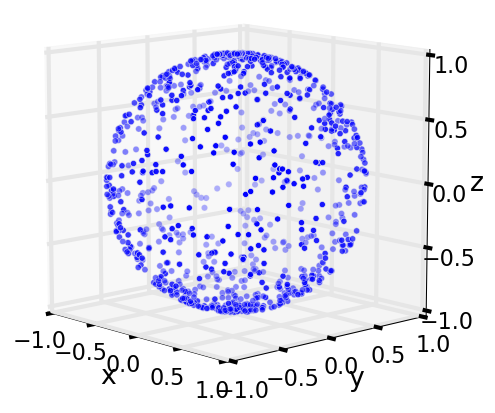
\includegraphics[width=0.49\textwidth]{appendix/img/badrandom.png}
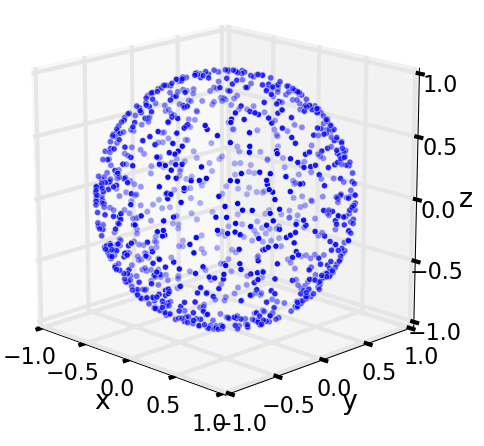
\includegraphics[width=0.49\textwidth]{appendix/img/goodrandom.png}
\caption{\textit{Left: }Illustration of a uniform sampling in angles $\phi$ and $\theta$ that doesn't give a uniform spherical distribution. \textit{Right: }Illustration of a good spherical distribution.}
\label{fig:sphere}
\end{figure}

\noindent The differential surface area, $dA$, is equal to $dA(d\phi,d\theta) = r^2 \sin(\phi) d\phi d\theta$. If we want the distribution $f(v)$ to be constant for a uniform distribution, then $f(v) = \frac{1}{4\pi}$ since $\int \int_S f(v)dA = 1$ and $\int \int_S dA = 4\pi$. We want the distribution in function of the angles, so

\begin{equation}
f(v)dA = \frac{1}{4\pi} dA = f(r) f(\phi,\theta)d\phi d\theta.
\end{equation}

\noindent Since we know the expression for $dA$, we find that

\begin{equation}
f(\phi,\theta) = \frac{1}{4\pi} \sin(\phi),
\end{equation}
and separating the angles:

\begin{alignat}{2}
f(\theta) =&& \int^\pi_0 f(\phi,\theta)d\phi = \frac{1}{2\pi}, \\
f(\phi)   =&& \int^{2\pi}_0 f(\phi,\theta)d\theta = \frac{\sin(\phi)}{2},
\end{alignat}
\noindent where it is clear that $f(\phi)$ scales with $\sin(\phi)$; there are more points needed at the equator (this makes sense, as the surface at the equator is much larger!).\\

\noindent The question is now how one can get a sample to follow the distribution of $f(\phi)$. For this, we use the \textit{inverse transform sampling} method where one makes use of the cumulative distribution function, $F(\phi)$, which increases monotonically

\begin{equation}
F(\phi) = \int^\phi_0 f(\phi')d\phi' = \frac{1}{2} \left(1-\cos(\phi)\right).
\end{equation}

\noindent The method shows that if $u$ is a random variable drawn from a uniform distribution, we have to find the inverse function of $F$,

\begin{align}
F(F^{-1}(u)) =& u \\
\frac{1}{2} \left(1-\cos(F^{-1}(u))\right) =& u\\
F^{-1}(u) =& \arccos(1-2u).
\end{align}

\noindent In other words: if $u$ is a random variable drawn from a uniform distribution, then $\phi = \arccos(1-2u)$ follows a distribution necessary for a uniform spherical distribution. Similarly, $\theta = \frac{1}{2\pi} u$.
\section{Power law distributions}
\label{sec:powerlawdistr}
Analogous to what was written in the previous section, one can produce a power law distribution from random numbers using the inverse transform sampling method: 
\begin{equation}
\begin{split}
f(E) &= A\cdot E^{-\gamma} \rm\ \ \ (power law)\\
F(E) &= \int^{E}_{E_{min}} A \cdot E^{-\gamma} dE = u \text{\ \ (inverse sampling, u random number [0,1])}\\
&= A \left[\frac{E^{-\gamma+1}}{-\gamma+1}\right]^E_{E_{min}}\\
&= \frac{A}{-\gamma+1}\left(E^{-\gamma+1}-E_{min}^{-\gamma+1}\right)\\
\end{split}
\end{equation}
\vspace{3mm}
\noindent Because we know that $F\left(F^{-1}(u)\right) = u$, we can find an expression for $F^{-1}(u)$:

\begin{equation}
\begin{split}
u &= \frac{A}{-\gamma+1}\left(\left(F^{-1}(u)\right)^{-\gamma+1}-E_{min}^{-\gamma+1}\right)\\
&\Rightarrow \\
            F^{-1}(u) &= \left(\left(\frac{-\gamma+1}{A}\cdot u\right)+ E_{min}^{-\gamma+1}\right)^{1/(-\gamma+1)}\\
\end{split}.
\end{equation}
To find $A$, we use the property of a CDF:
\begin{equation}
F(E_{max}) = 1\Rightarrow A = \frac{-\gamma+1}{E_{max}^{-\gamma+1}-E_{min}^{-\gamma+1}},
\end{equation}
\noindent leading to
\begin{equation}
F^{-1}(u) = \left((1-u) \cdot E_{min}^{-\gamma+1} + u \cdot E_{max}^{-\gamma+1}\right)^{1/(-\gamma+1)},
\end{equation}
\noindent which shows how one can draw a distribution in function of $E$ following $f(E)$ with a uniform random number $u$.\\

\noindent For $\gamma$ = -1, the computations are analogous and one can see that this will produce a uniform distribution in log space. This is shown in Figure \ref{fig:powerlawrandom}.
            \begin{equation}
            \begin{split}
            E &= E_{min} \cdot 10^{u\cdot \log{\frac{E_{max}}{E_{min}}}}\\
            &= 10^{u[\log{E_{min}},\log{E_{max}}]}
\end{split}
\end{equation}
            
\begin{figure}
\centering
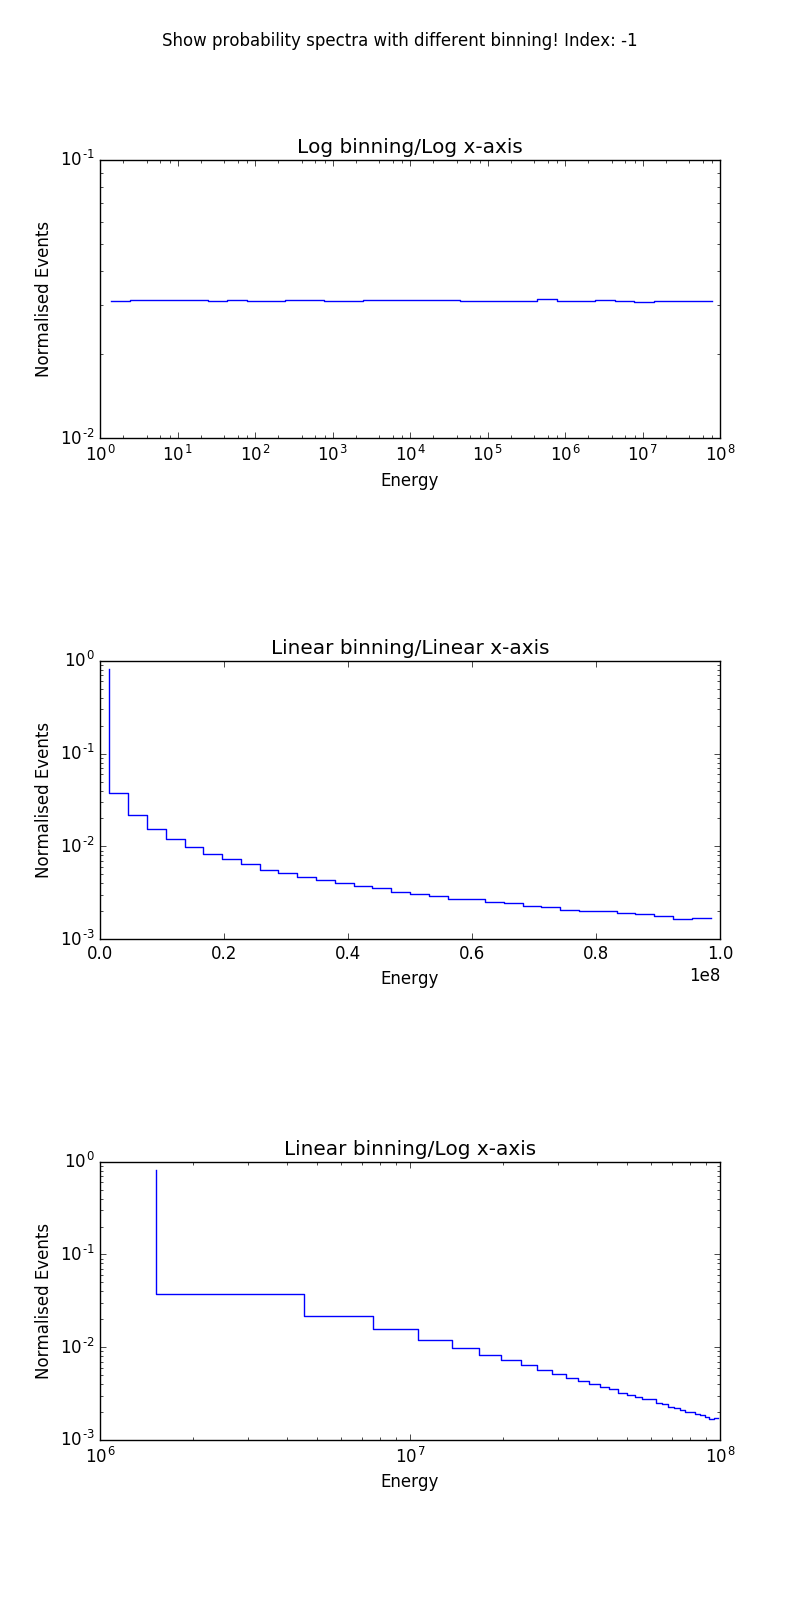
\includegraphics[width=0.48\textwidth]{appendix/img/probabilitypowerlaw_index1}
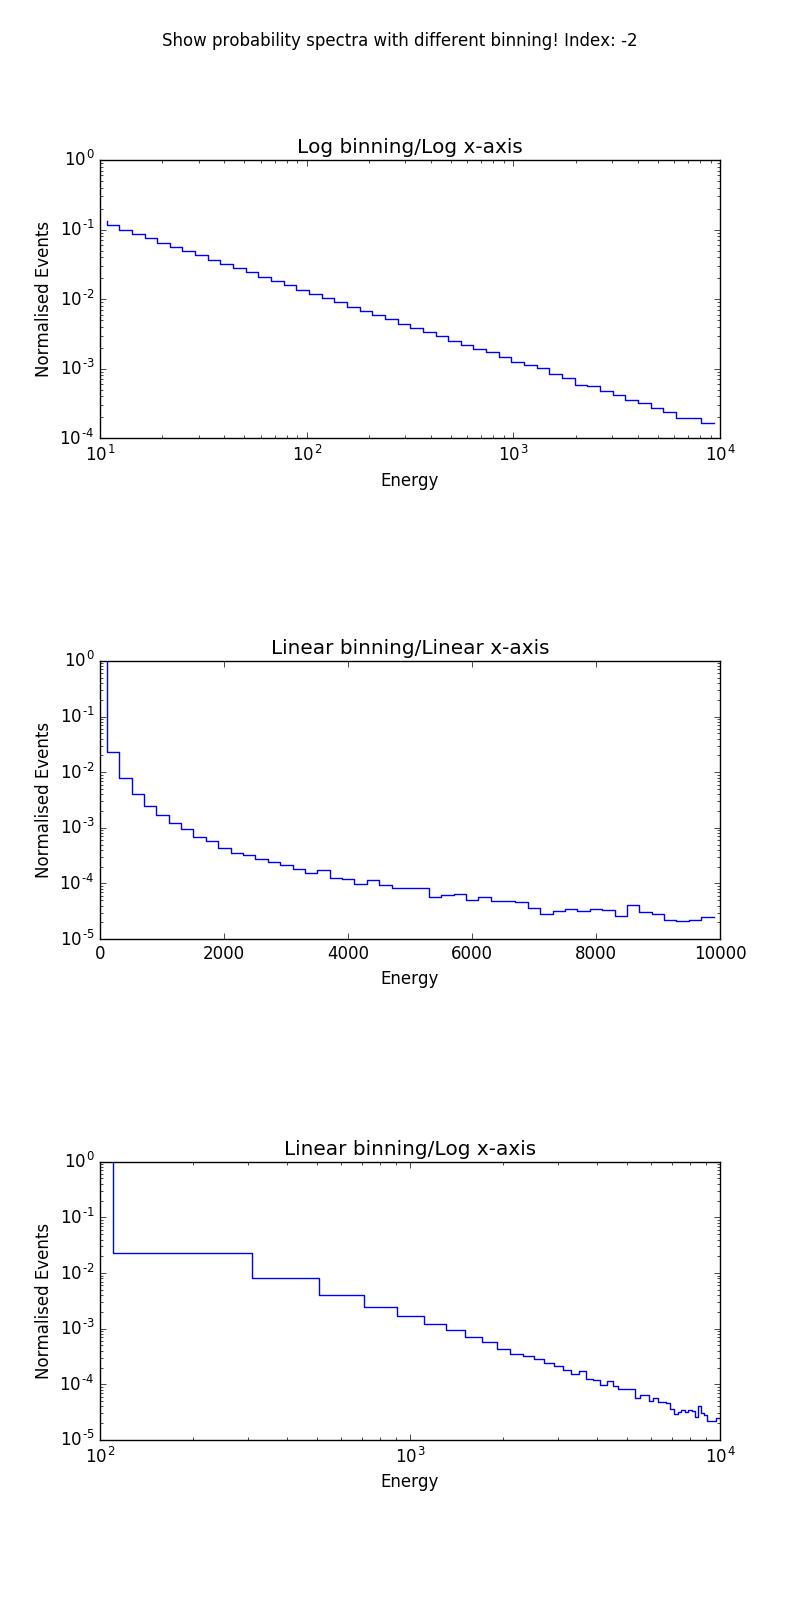
\includegraphics[width=0.48\textwidth]{appendix/img/probabilitypowerlaw_index2}
\caption{\textit{Left: }Histograms with different binnings showing the behavior of an energy spectrum with spectral index -1. \textit{Right: }Histograms with different binnings showing the behavior of an energy spectrum with spectral index -2.}
\label{fig:powerlawrandom}
\end{figure}

In Figure \ref{fig:signalweighting} the signal reweighting is shown.

\begin{figure}
\centering
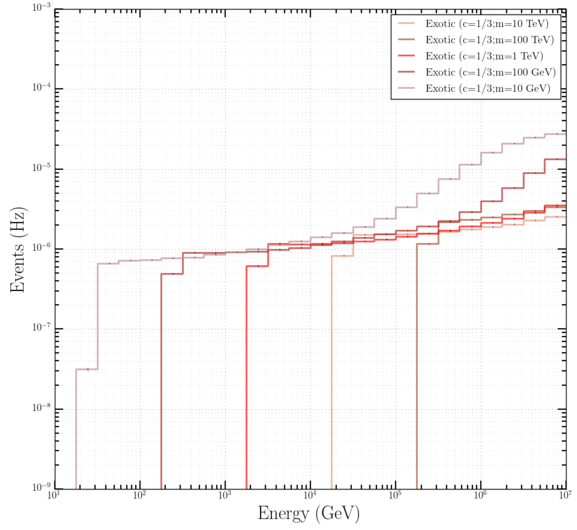
\includegraphics[width=0.48\textwidth]{appendix/img/SpectrumBeforeWeighting.png}
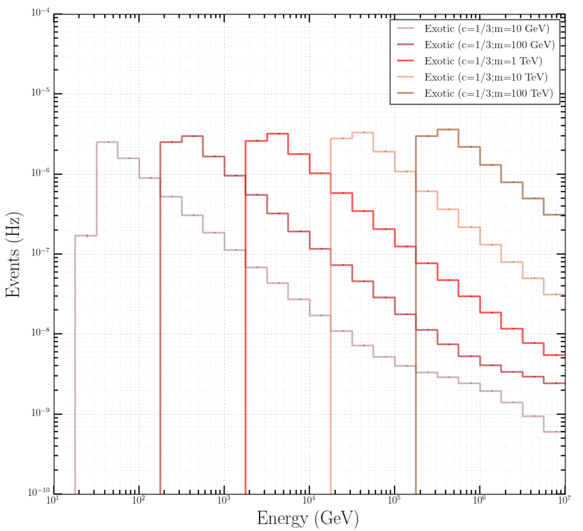
\includegraphics[width=0.48\textwidth]{appendix/img/SpectrumAfterWeighting.png}
\caption{\textit{Left: }Spectrum of the signal before weighting following an $E^{-1}$ spectrum. The rise in the rate in function of energy is due to the trigger efficiency that increases in function of energy. \textit{Right: }Spectrum of the signal after reweighting to an energy spectrum of $E{-2}$.}
\label{fig:signalweighting}
\end{figure}

\section{Angular distributions}
\label{sec:angularappendix}
As seen in Section \ref{sec:sphericalrandom}, the differential space angle $d\Omega$ is equal to

\begin{equation}
d\Omega = \sin(\theta) d\theta d\phi.
\end{equation} 

\noindent If one shows the distribution of $\phi$ and/or $\theta$, then this is the same as showing partial integrations per bin. We find that

\begin{equation}
\Omega \propto \cos(\theta),
\end{equation}

\noindent or in other words: the space angle is proportional to the azimuth and the cosine of the zenith. An example is shown in Figure \ref{fig:spaceangle}.

\begin{figure}
\centering
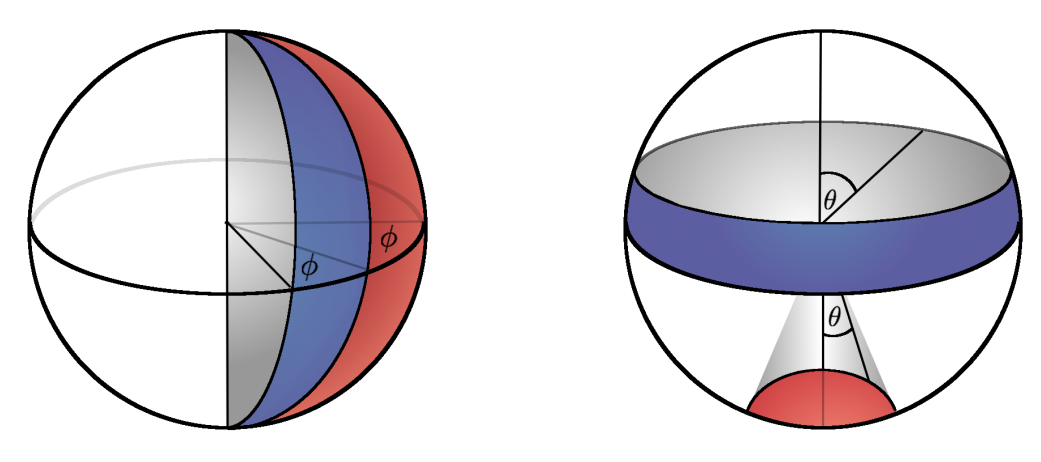
\includegraphics[width = 0.8\textwidth]{appendix/img/spaceangle.png}
\caption{Illustration of angle distributions in spherical coordinates. The blue and red surfaces are equal in size. The left figure clearly shows the surface to be proportional to the azimuth. The right figure shows how there is a non-trivial dependence on the zenith angle for equal partitions on the surface of a sphere.}
\label{fig:spaceangle}
\end{figure}

\section{Weighting}
\label{sec:weighting}
A method that is often used in simulations is \textit{weighting}. The simulated and expected differential flux of particles is often not the same, mainly due to two reasons:

\begin{itemize}
\item The flux has no uniform power law behavior. As can bee seen in Figure \ref{fig:spectrumCR}, there can be multiple ``kinks'' and changes in a spectrum. Instead of simulating the flux according to one model, a general uniform flux is used and later reweighted to be able to fit to other models more easily.
\item A steep power law indicates very few events at the highest energy bins. This means large CPU time would be necessary to simulate these events. As an example, let us assume two different fluxes

\begin{equation}
f_1 = A \cdot x^{-1},
\end{equation}

\begin{equation}
f_2 = B \cdot x^{-2},
\end{equation}
\noindent where $A = 10^3$ and $B = 10^4$, so the fluxes cross at a value of $x^{-1+2} = x = \frac{10^4}{10^3} = 10$. In the interval $x \in [10^3,10^4]$, the number of events for $f_1$ is equal to $10^3$, whereas for $f_2$ this is equal to 9.\\

\noindent Simulating with harder spectra\footnote{Harder spectra equals to a lower gamma, since there will be more high-energy events.} leads to more statistics in high-energy bins.
\end{itemize}
\vspace{3mm}
\noindent The weights can be generally written down as

\begin{equation}
w = \frac{dN_{exp}}{dA d\Omega dE dt} \times \frac{dA d\Omega dE}{dN_{sim}}.
\end{equation}

\vspace{3mm}
\noindent A disadvantage of using weights is that certain events with a high weight are rare but can dominate or obscure the sample in the tails of certain distributions.

\chapterimage{lines.jpg}
\chapter{Boosted Decision Trees: examples}
\label{ch:adaboostappendix}

\section{Decision Tree: simple example}
Let us assume we want to categorize 6 people if they are \textit{healty} or \textit{unhealthy}. The decision tree training can be done if we have a sample set that labels people in these two categories and some other information about these persons is known. In this example, we know if the person is older than 30, if he eats a lot of pizza and if he exercises a lot. This is summarized in Table \ref{tab:pizza}.\\

\begin{table}[t]
\centering
\caption{Summary of dataset used to train decision tree.}
\label{tab:pizza}
\begin{tabular}{|l|c|c|c|r|}
\hline
\rowcolor[HTML]{F1A91E} 
Person & Age \textless 30 & Eats lots of pizza & Exercises often & Healthy \\ \hline
A & 1 & 1 & 1 & 0 \\ \hline
B & 1 & 0 & 1 & 1 \\ \hline
C & 1 & 0 & 0 & 1 \\ \hline
D & 0 & 0 & 0 & 0 \\ \hline
E & 0 & 0 & 1 & 1 \\ \hline
F & 0 & 0 & 1 & 1 \\ \hline
\end{tabular}
\end{table}

\noindent As an example, we can show how the first child nodes are determined. The sample set has three variables and the variable selection that allows for the largest separation (see Eq. \ref{eq:separationgain}) will be chosen. The results from $\Delta S$ for the age, pizza and exercises selections are 0, -1.7 and -2.6 respectively. Therefore, it should be clear that the age selection should be chosen first in the decision tree as it gives the larges separation for the child nodes. Deeper child nodes are selected in a similar fashion. 

\section{AdaBoost: simple example}
Consider a binary decision tree classification with 10 training examples. The illustrations below are 2D variable distributions.\\
\newline
\noindent We give each event an equal weight, making the weight distribution $D_1$ uniform. For this simple example, each of our classifiers will be an axis-parallel linear classifier (simple cut in one of the two variables).

\paragraph{Initial distribution}


\begin{center}
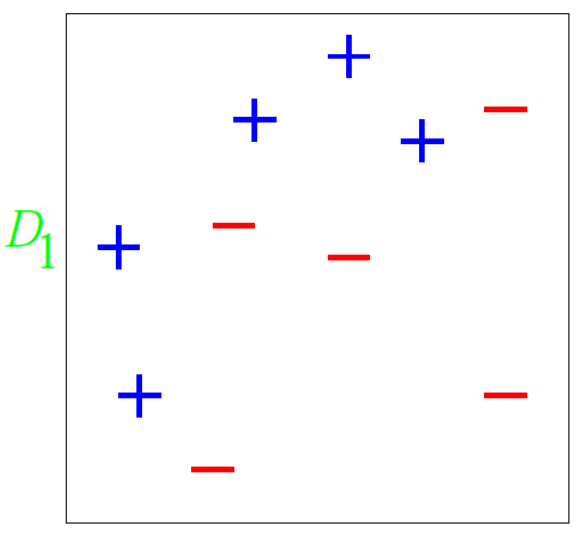
\includegraphics[width=7cm]{appendix/img/adaboost1.png}
\end{center}

\paragraph{Round 1}
\begin{center}
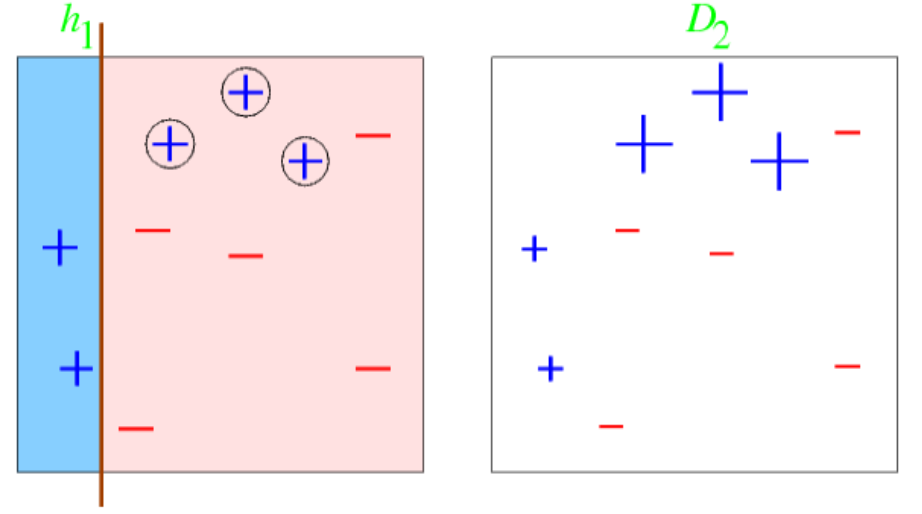
\includegraphics[width=7cm]{appendix/img/adaboost2.png}
\end{center}

\begin{itemize}
\item Error rate of $h_1$: $\epsilon_1 = 0.3$; weight of $h_1$ (see Eq. \ref{eq:boostfactor}): $\alpha_1 = \frac{1}{2} \ln\left(\frac{1-\epsilon_1}{\epsilon_1}\right) = 0.42$
\item An event that is misclassified gets a higher weight: weight multiplied with $\exp(\alpha_1)$
\item An event that is correcly classified gets a lower weight: weight multiplied with $\exp(-\alpha_1)$
\end{itemize}

\paragraph{Round 2}

\begin{center}
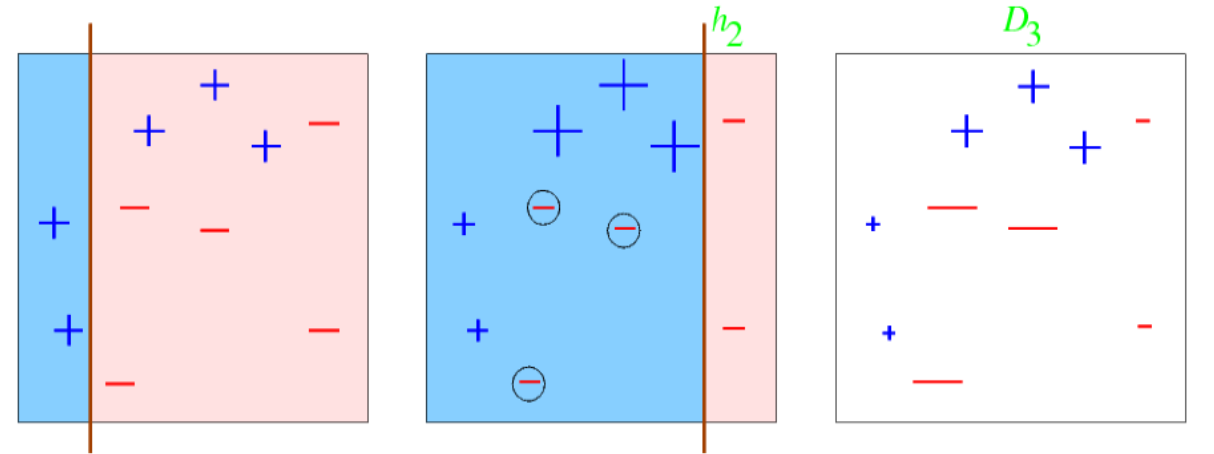
\includegraphics[width=7cm]{appendix/img/adaboost3.png}
\end{center}

\begin{itemize}
\item Error rate of $h_1$: $\epsilon_1 = 0.21$; weight of $h_2$ (see Eq. \ref{eq:boostfactor}): $\alpha_2 = \frac{1}{2} \ln\left(\frac{1-\epsilon_2}{\epsilon_2}\right) = 0.65$
\item An event that is misclassified gets a higher weight: weight multiplied with $\exp(\alpha_2)$
\item An event that is correcly classified gets a lower weight: weight multiplied with $\exp(-\alpha_2)$
\end{itemize}

\paragraph{Round 3}

\begin{center}
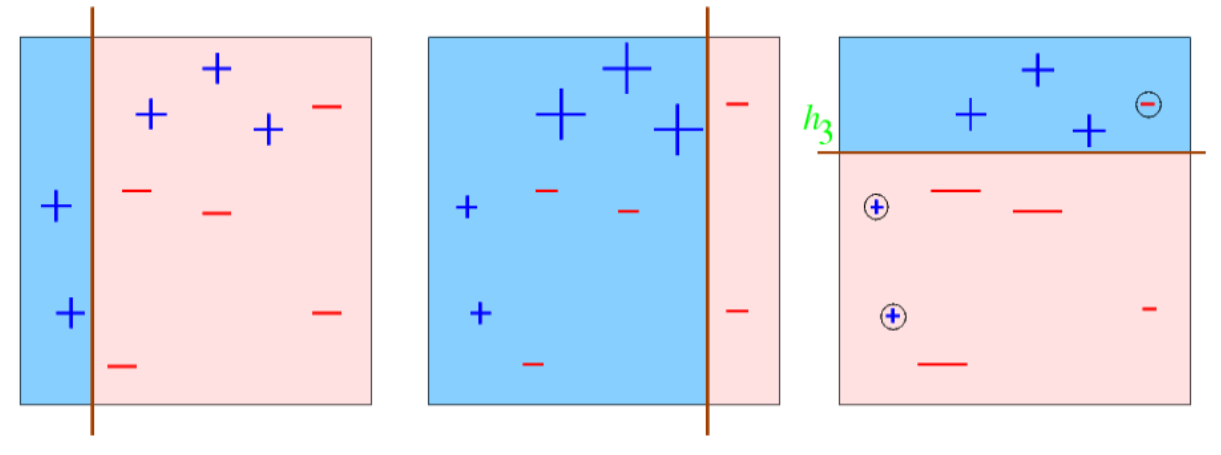
\includegraphics[width=7cm]{appendix/img/adaboost4.png}
\end{center}

The error rate of $h_1$: $\epsilon_1 = 0.21$; weight of $h_2$ (see Eq. \ref{eq:boostfactor}): $\alpha_2 = \frac{1}{2} \ln\left(\frac{1-\epsilon_2}{\epsilon_2}\right) = 0.65$

Let us suppose to stop after this round, we now have a forest of 3 decision classifiers: $h_1,h_2,h_3$.

\paragraph{Final step}
The final classifier is a weighted linear combination of all the classifiers:


\begin{center}
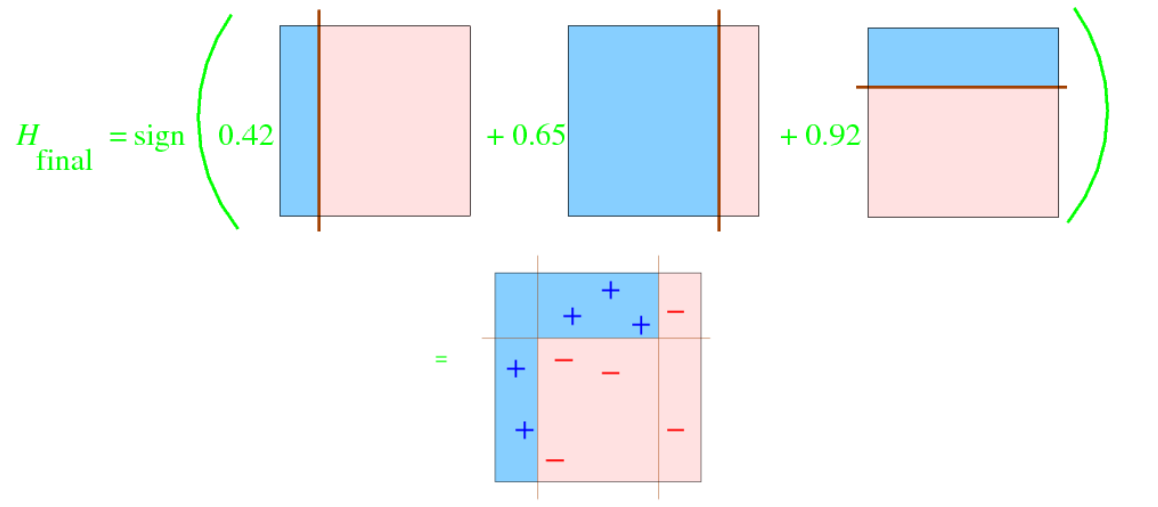
\includegraphics[width=12cm]{appendix/img/adaboost5.png}
\end{center}

\usechapterimagefalse
\chapterimage{whitepage.png}
\chapter{Resampling Methods}
\label{ch:resampling}
\usechapterimagetrue

Resampling is a method used in statistical analyses and commonly refers to methods that extract information from a larger set by taking subsets and performing significance or validation tests. Two common examples are \textit{bootstrapping} and \textit{cross-validation} and are explained below.

\section{Bootstrapping}
The basic idea of bootstrapping is that we can draw conclusions from a certain sample in a larger, unknown, population by taking a subsample and performing inference about the sample from the subsample. The method assumes that the true probability distribution from a sample to a population can be reasonably estimated from an emperical probability distribution from a subsample to a sample.

Assume we have a total population $P$ of size $N_P$ and a measured sample $N$ of size $N_N$, where 

\begin{equation}
N_N < N_P \textrm{ and } N \subset P.
\end{equation}
From $N$, only one estimate of the mean can be computed. To get a sense of the variability one could assume a Gaussian or Poissonian probability, or what is done in this method: form a new subsample that is also of size $N_N$. This can only be done by \textit{sampling with replacement} where the elements in the subsample can be repeated. If $N_N$ is sufficiently large, this will almost certainly result in subsamples that are different from the original sample. The mean can be computed from the new subsample and this process is repeated a large number of times (typically of the order of 1,000). The distribution of the means then indicates our confidence in the sample mean where a large variability assumes large uncertainties.

\section{Cross-validation}
Another example of a resampling method is cross-validation, sometimes called \textit{rotation estimation}, where one wants to estimate the predictive power of a model. From a sample, a subsample called the \textit{training sample} is selected to train a model (e.g. a BDT). This model is then checked on another subsample called the \textit{testing sample}. This allows to estimate how the model will generalize to other independent datasets. Training samples will often have a lower performance in parameter estimations from the testing sample than the training sample. In cross-validation one tries to get an estimate for this effect. An often used cross-validation method is called \textit{$k$-fold cross-validation}.

In this method, one iterates the procedure of selecting a training sample and a testing sample $k$ times. If the total size of the sample set is $N_N$, the testing samples will have a size of $N_N/k$. As we have $k$ iterations, the subsamples can be chosen without replacement and are unique each time. At each iteration, the training sample will have a size of $N_N - \frac{N_N}{k} = N_N \cdot \frac{k-1}{k}$. The $k$ results can then be averaged to produce a single estimation.\\

\noindent Pull-validation is another example of a resampling method and is explained in more detail in Section \ref{subsec:pv}. Illustratively, it can be visualized as in Figs. \ref{fig:pvillustration1} and \ref{fig:pvillustration2}.

\begin{figure}
\centering
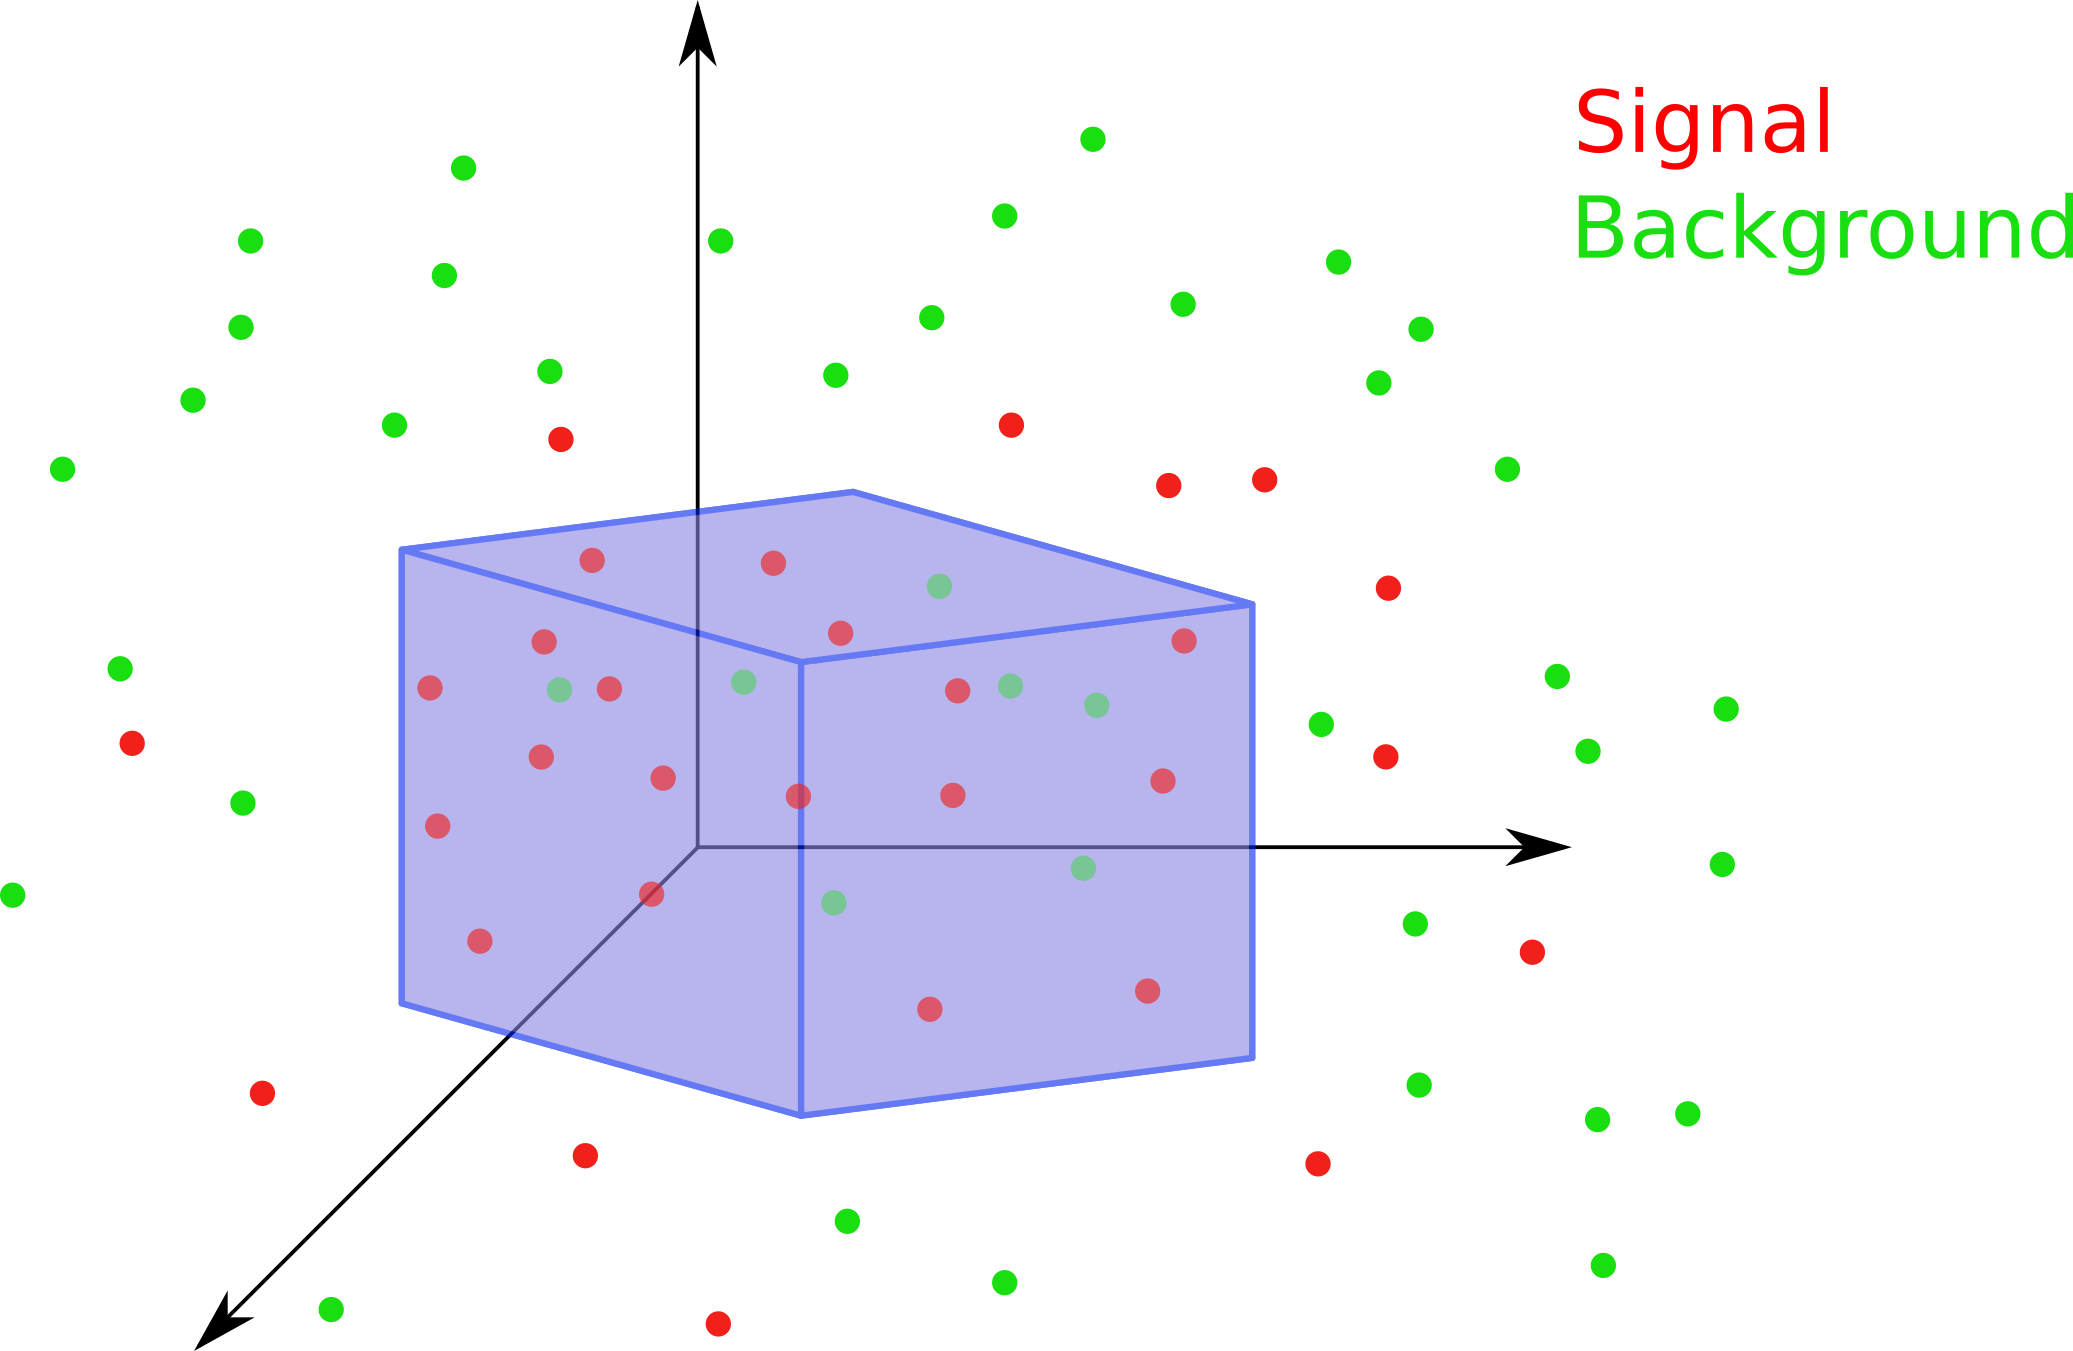
\includegraphics[width=0.49\textwidth]{appendix/img/resampling_before.png}
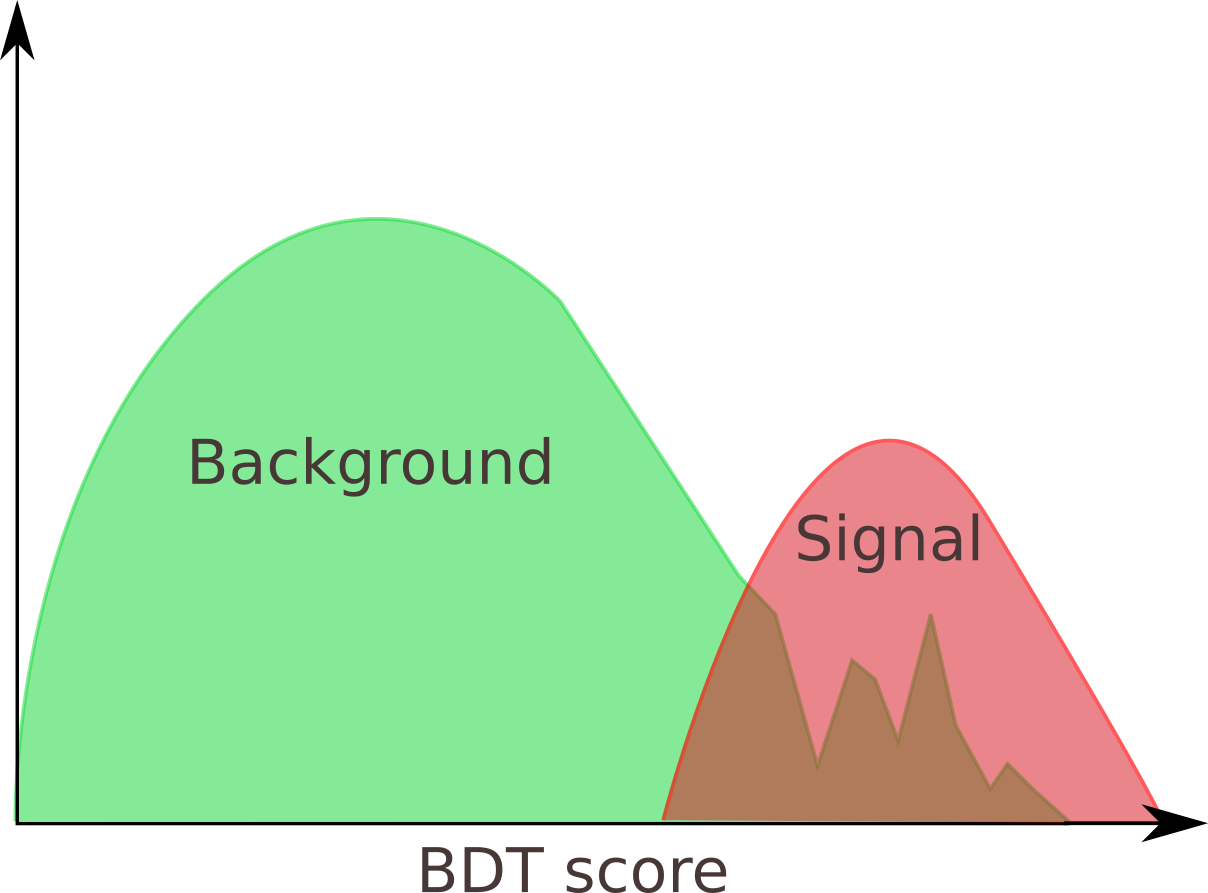
\includegraphics[width=0.49\textwidth]{appendix/img/hist1.png}
\caption{Simplistic llustration of parameter space that originates from one branch in one BDT. The axes represent physical parameters that are used in the BDT. The blue box illustrates an example of cuts that are placed on the parameters. The BDT algorithm converts the survival probability of an event regarding these cuts into a score. Limited statistics for the background events are represented by a discontinuous tail.}
\label{fig:pvillustration1}
\end{figure}

\begin{figure}
\centering
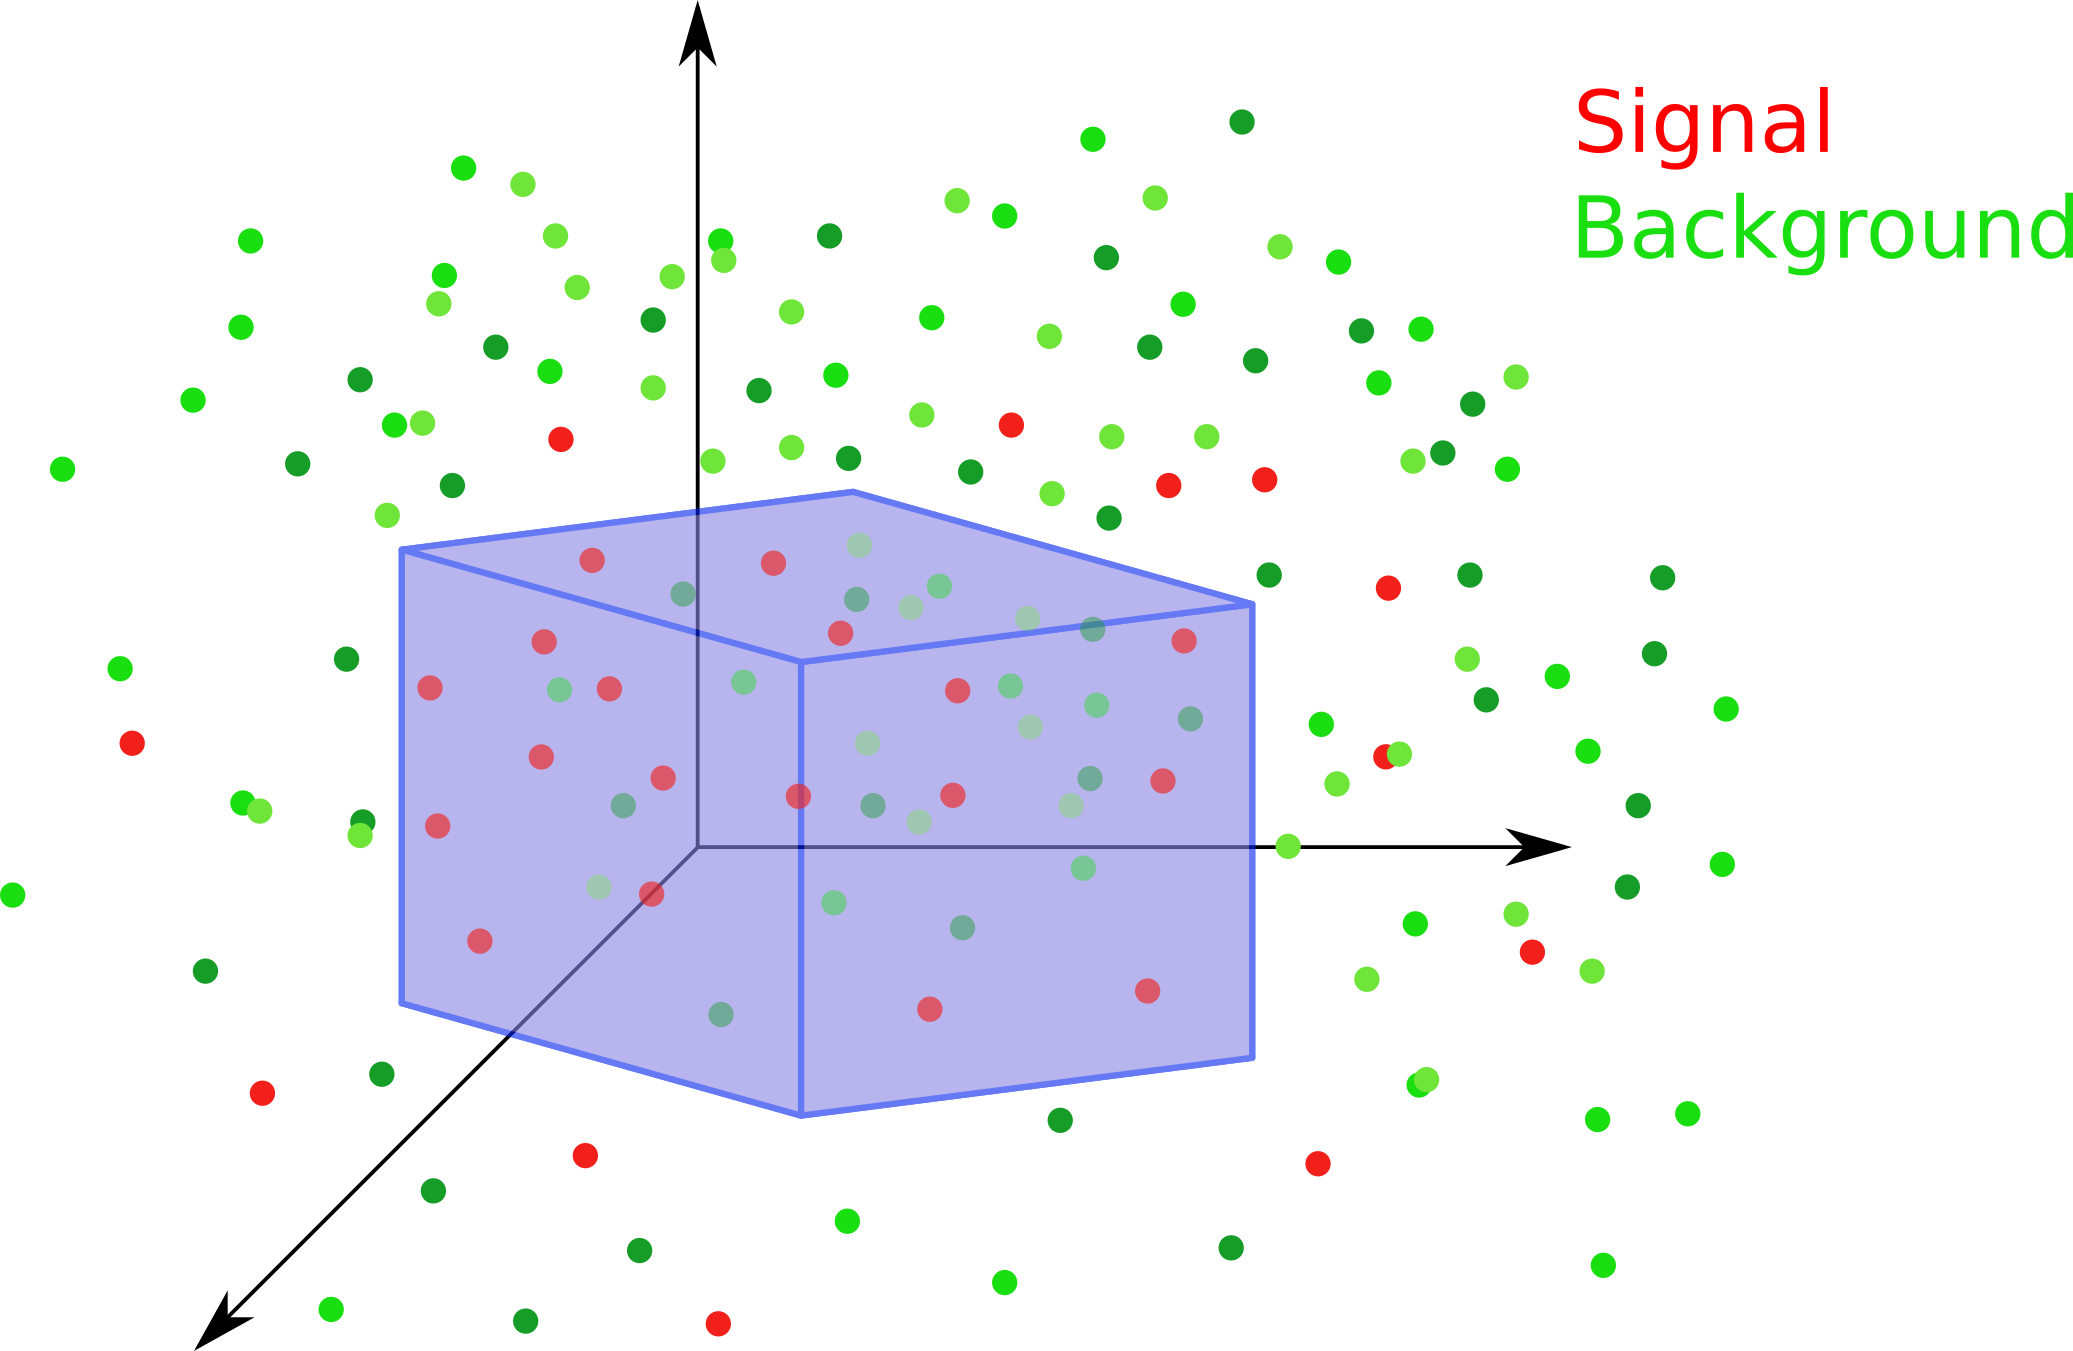
\includegraphics[width=0.49\textwidth]{appendix/img/resampling_after.png}
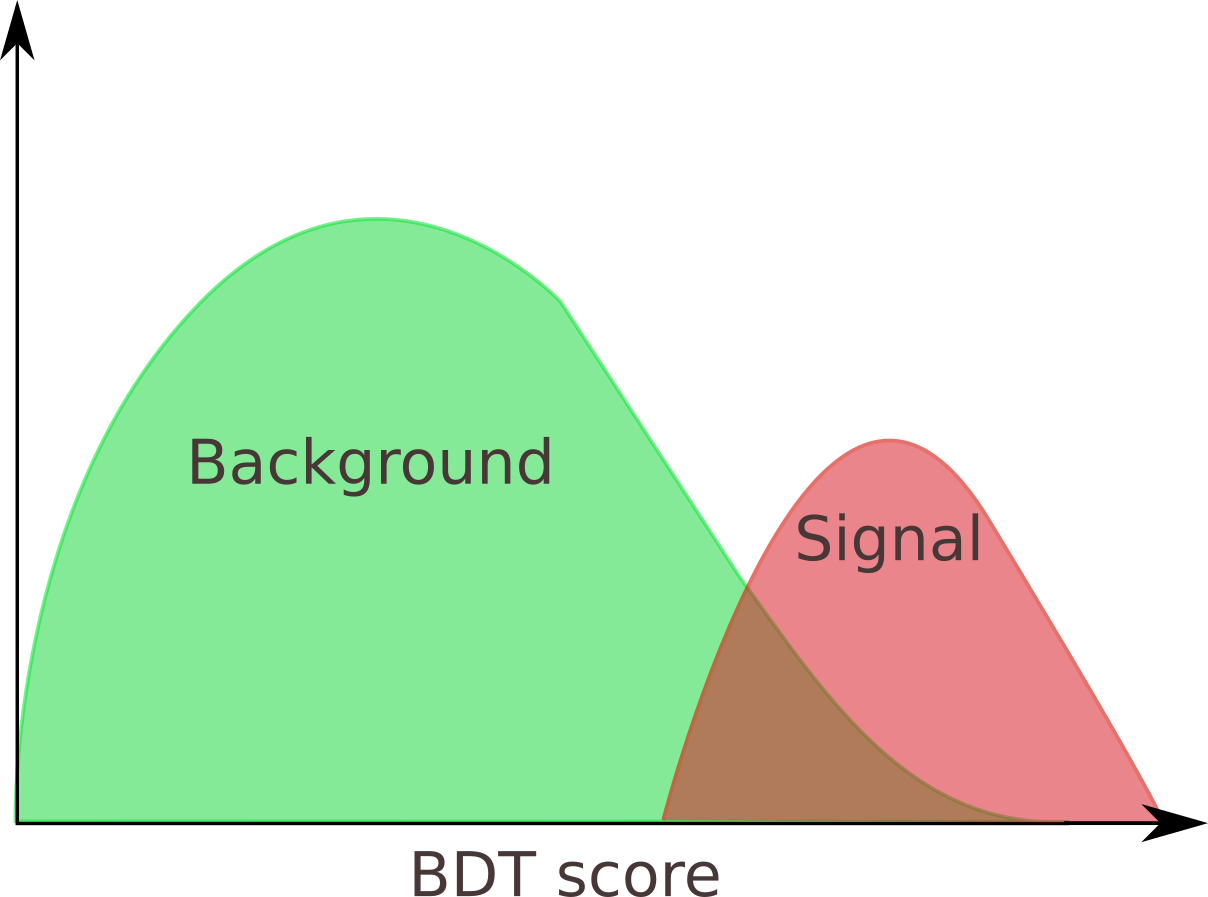
\includegraphics[width=0.49\textwidth]{appendix/img/hist2.png}
\caption{Simplistic llustration of parameter space that originates from one branch in one BDT. Resampling the background (different green points) results in more statistics in the tail.}
\label{fig:pvillustration2}
\end{figure}

\usechapterimagefalse
\chapterimage{whitepage.png}
\chapter{Additional BDT Checks}
\label{ch:bdtchecks}
\usechapterimagetrue
As explained in Section \ref{sec:BDT}, it is important to perfom some checks to see if a BDT is performing normally. A first check is done to see if the distribution of the training and testing samples show significant differences. This is shown in Figure \ref{fig:overtraining} and explained in more detail in Section \ref{subsec:overtraining}.\\

\begin{figure}[ht]
\centering
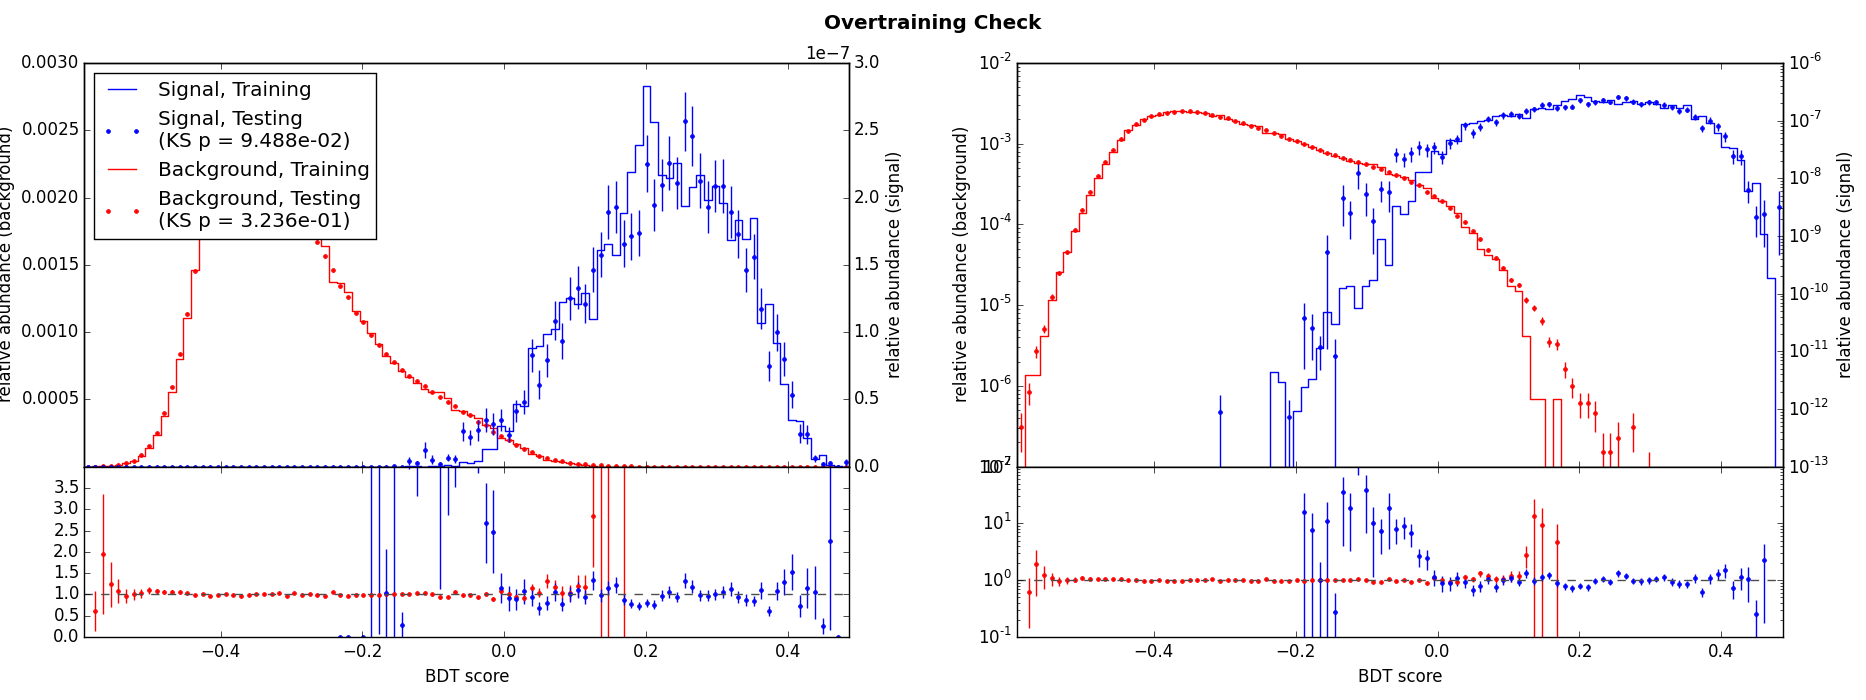
\includegraphics[width=\textwidth]{appendix/img/overtrain.png}
\caption{No significant overtraining seems to be present in signal and background. The signal used here is an SMP of charge $\frac{1}{2}$ and mass 100 GeV.}
\label{fig:overtraining}
\end{figure}

\noindent The correlation between the 17 variables that were used in the BDT is shown in Figure \ref{fig:correlation}. These variables were selected with the mRMR feature, which shows an excellent performance since there are no significant correlations in both signal and backround visible.
\begin{figure}[ht]
\centering
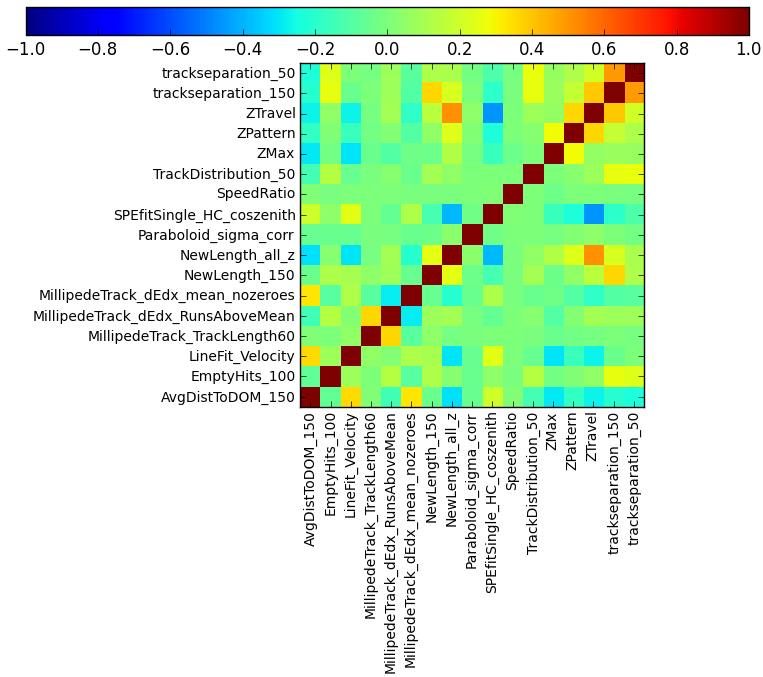
\includegraphics[width=0.49\textwidth]{appendix/img/correlationbackground.png}
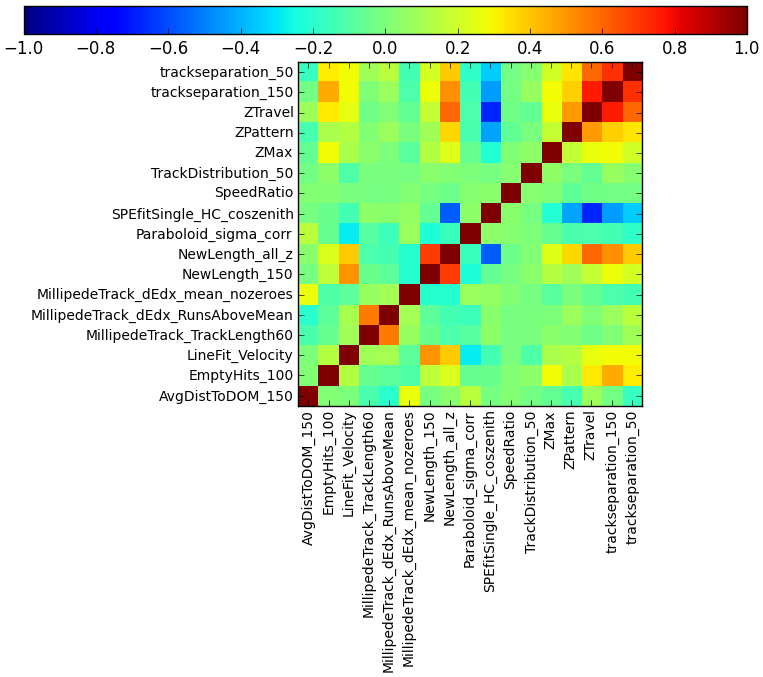
\includegraphics[width=0.49\textwidth]{appendix/img/correlationsignal.png}
\caption{Here we see the correlation between the variables that are used in the BDT. There is no significant correlation in \textit{both} signal and background, making these variables appropriate to use.}
\label{fig:correlation}
\end{figure}


\usechapterimagefalse
\chapterimage{whitepage.png}
\chapter{Data Events at Final Level}
\label{ch:eventviewerFinal}
\usechapterimagetrue

\begin{figure}
\centering
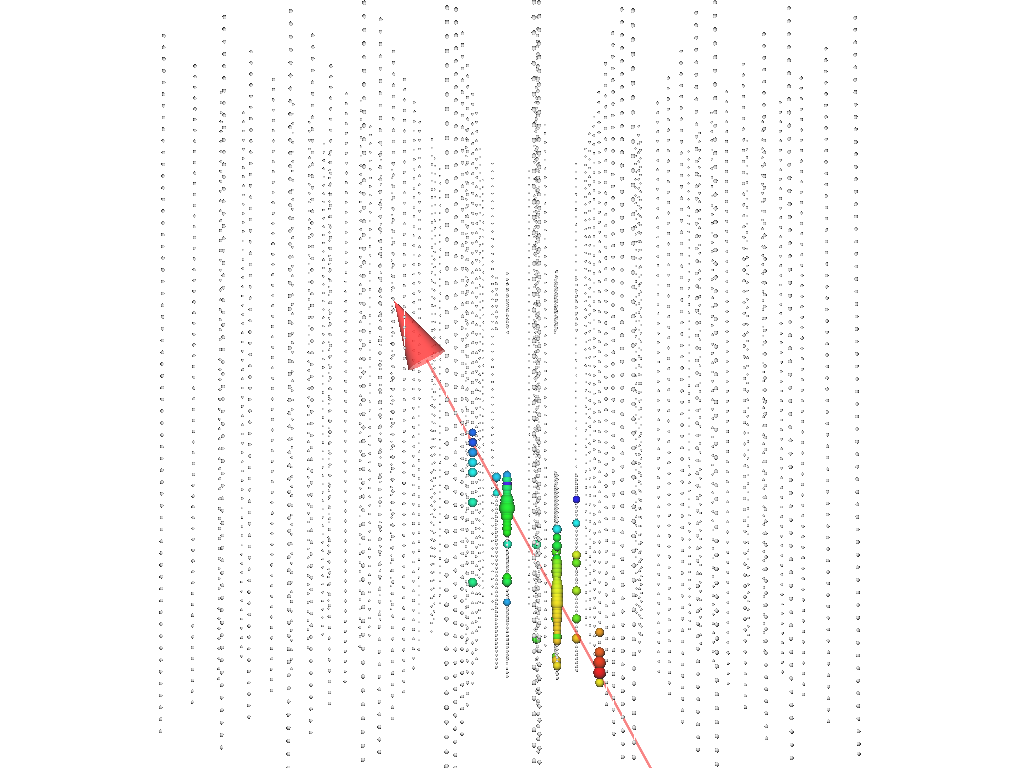
\includegraphics[width=0.49\textwidth]{appendix/img/FINAL_data_m_10000_ch1ovr2_1.png}
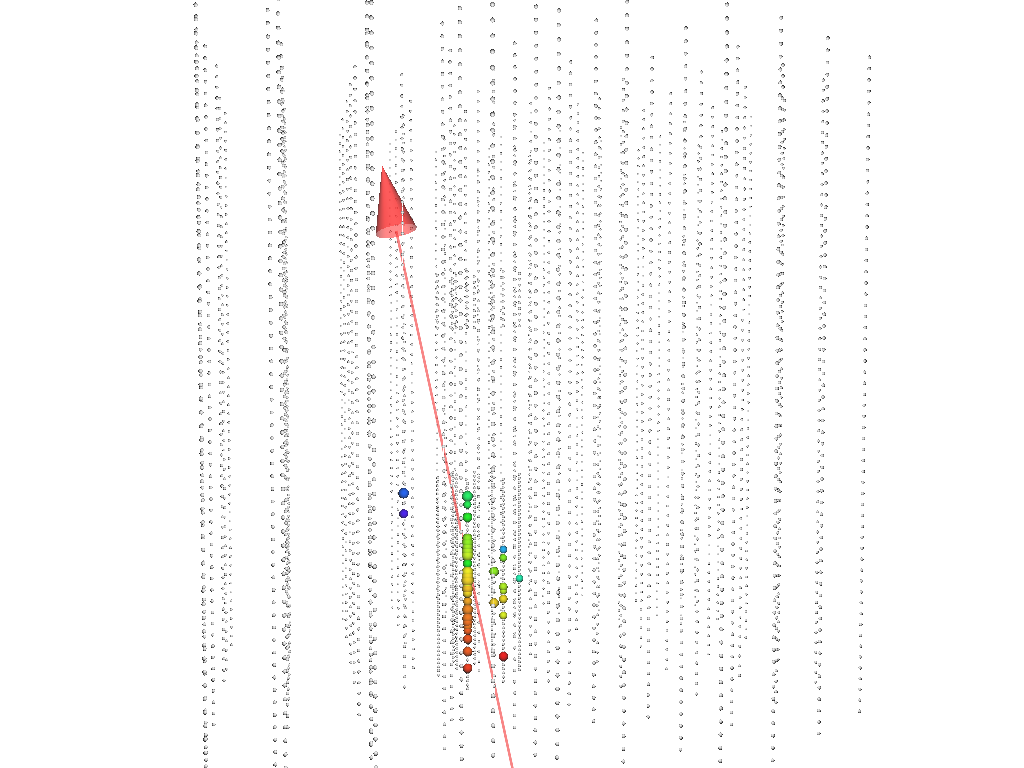
\includegraphics[width=0.49\textwidth]{appendix/img/FINAL_data_m_10000_ch1ovr2_1_NUMUANOLOGY.png}
\caption{Event viewers of an event that survive the SMP with mass 10 TeV and charge 1/2 selection. \textit{Left (real data): } Short and bright upgoing track corresponds to $\mu$ from an atmospheric $\nu_\mu$ that stopped shortly after leaving DeepCore. \textit{Right: }Simulated atmospheric $\nu_\mu$ event that strongly resembles this data event.}
\label{fig:final_1}
\end{figure}

\begin{figure}
\centering
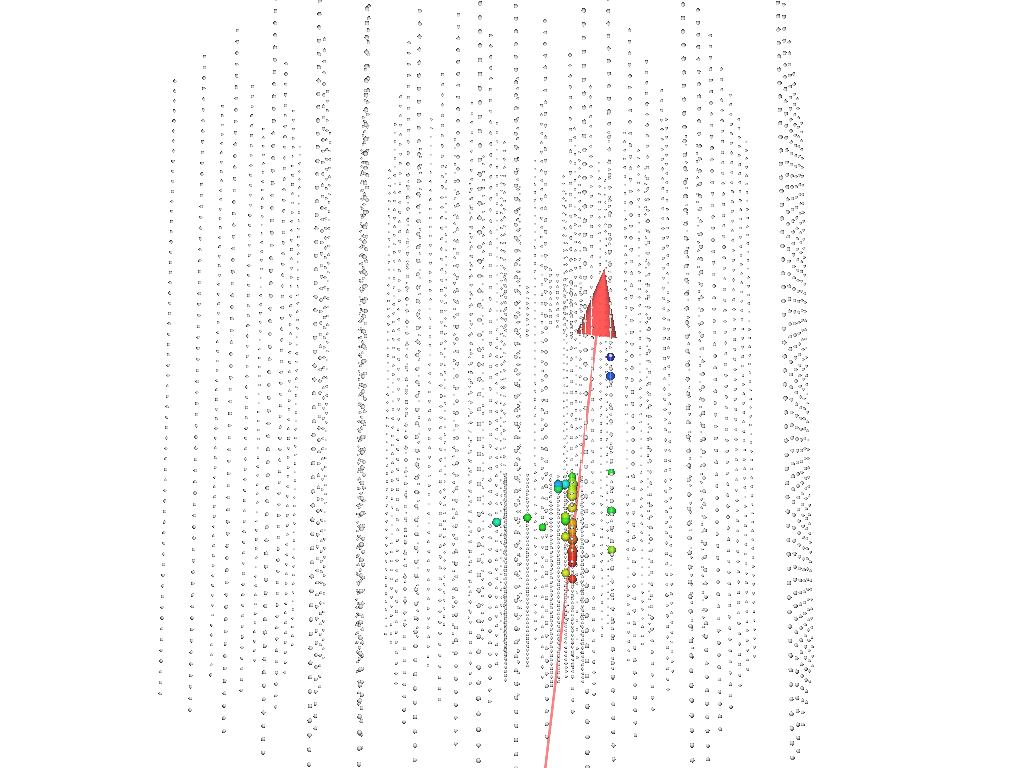
\includegraphics[width=0.49\textwidth]{appendix/img/FINAL_data_m_10000_ch1ovr2_2.png}
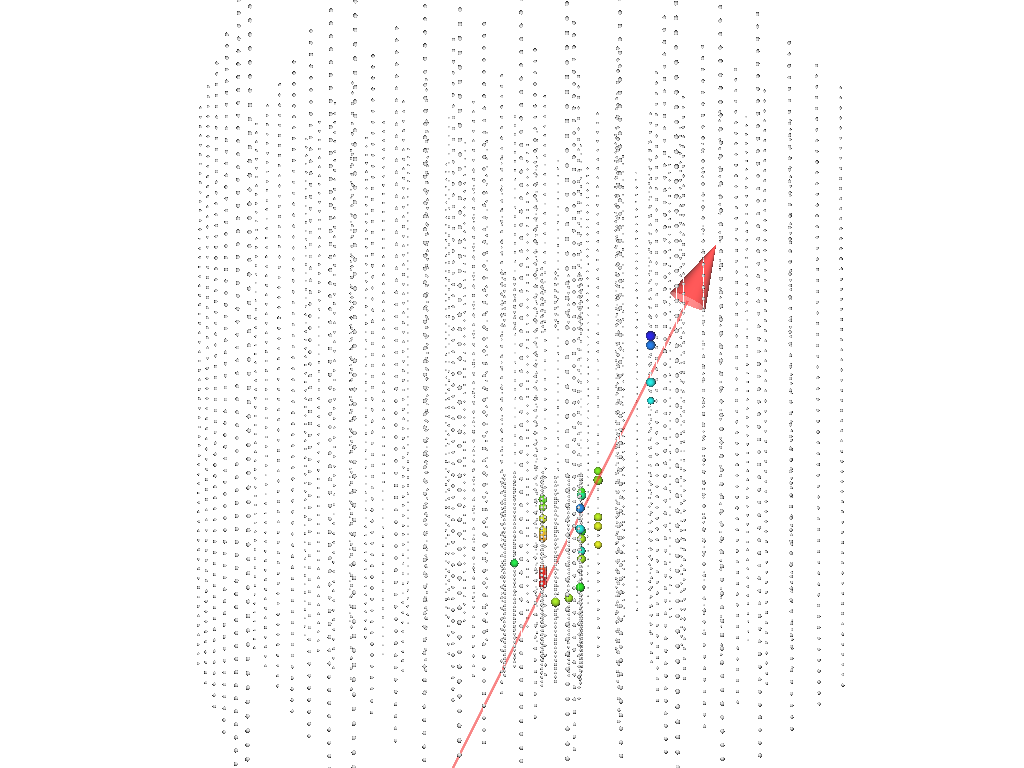
\includegraphics[width=0.49\textwidth]{appendix/img/FINAL_data_m_10000_ch1ovr2_2_NUMUANALOGY.png}
\caption{Event viewers of an event that survive the SMP with mass 10 TeV and charge 1/2 selection. \textit{Left (real data): }Corresponds to an upgoing $\mu$ from atmospheric $\nu_\mu$ that either starts or ``corridors'' in between strings and skims DeepCore along the side. After leaving DeepCore it only passes close to one string, giving the two hits. \textit{Right: }Simulated atmospheric $\nu_\mu$ event that strongly resembles this data event.}
\label{fig:final_1}
\end{figure}

\begin{figure}
\centering
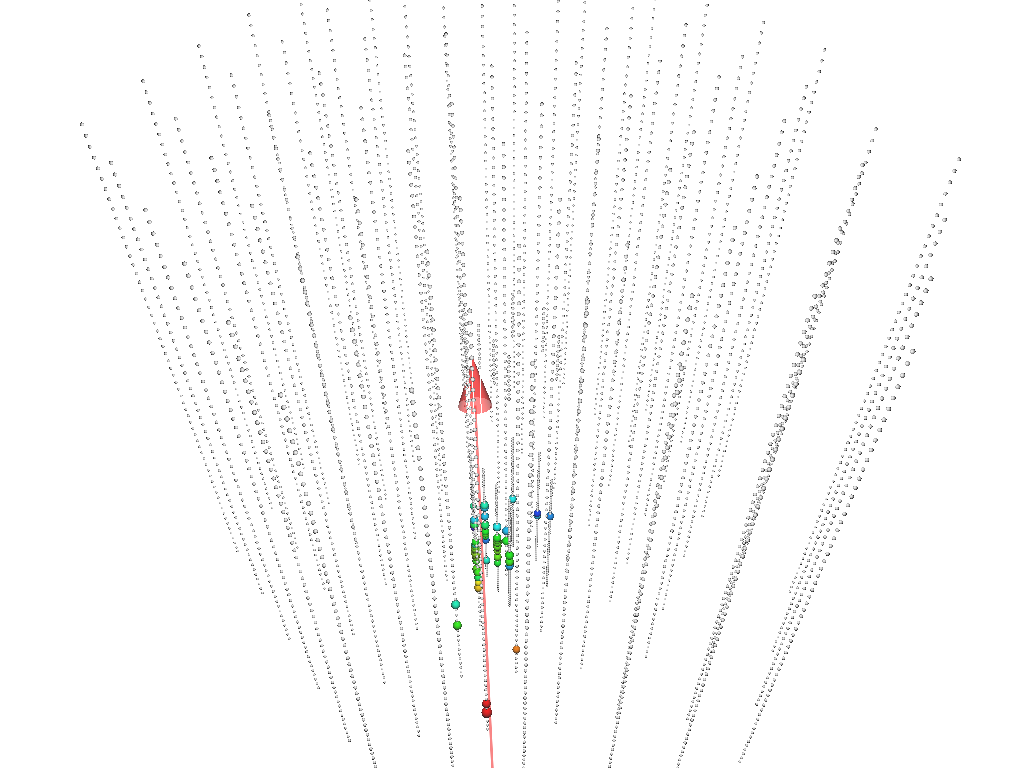
\includegraphics[width=0.49\textwidth]{appendix/img/FINAL_data_m_10_ch1ovr3_1.png}
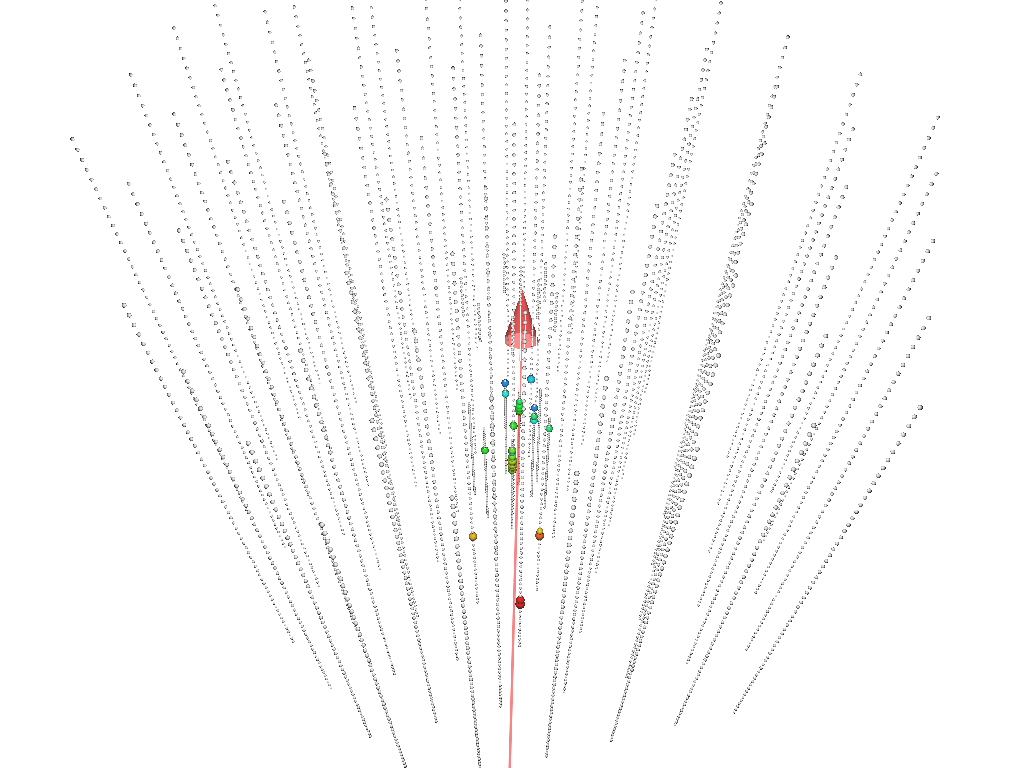
\includegraphics[width=0.49\textwidth]{appendix/img/FINAL_data_m_10_ch1ovr3_1_NUMUANALOGY.png}
\caption{Event viewers of an event that survive the SMP with mass 10 GeV and charge 1/3 selection. \textit{Left (real data): }Corresponds to a horizontal $\mu$ from atmospheric $\nu_\mu$ that passes close to one string in IceCube and stops in DeepCore where more light is recorded. \textit{Right: }Simulated atmospheric $\nu_\mu$ event that strongly resembles this data event.}
\label{fig:final_3}
\end{figure}

\begin{figure}
\centering
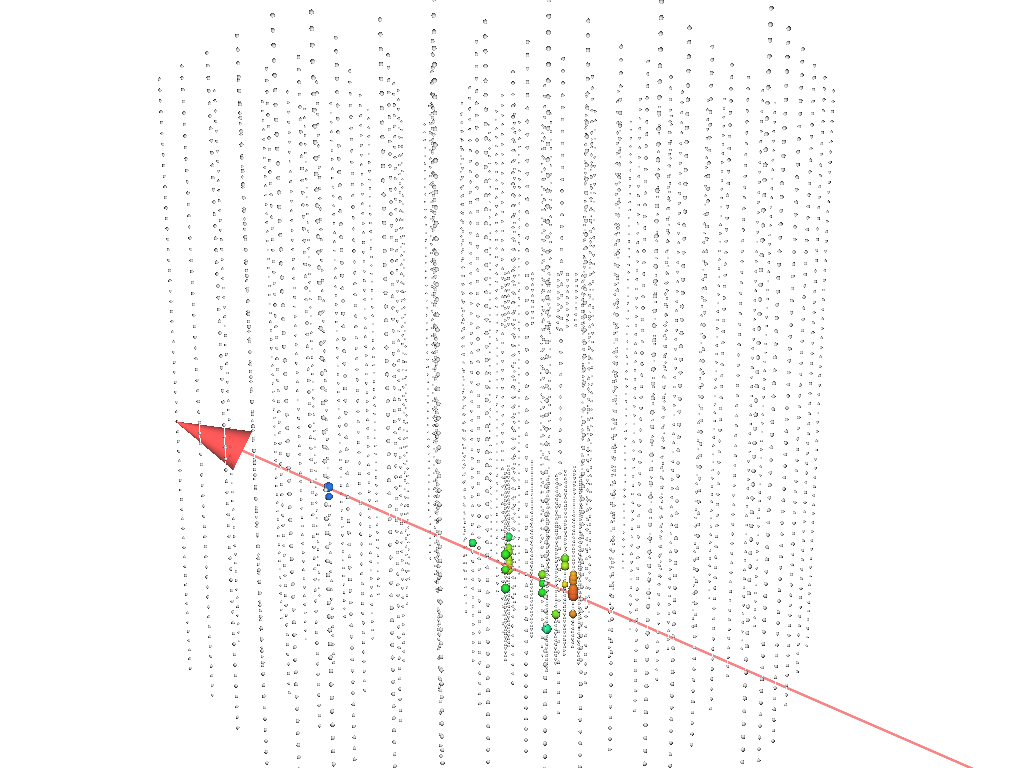
\includegraphics[width=0.49\textwidth]{appendix/img/FINAL_signal_m_100_ch1ovr2.png}
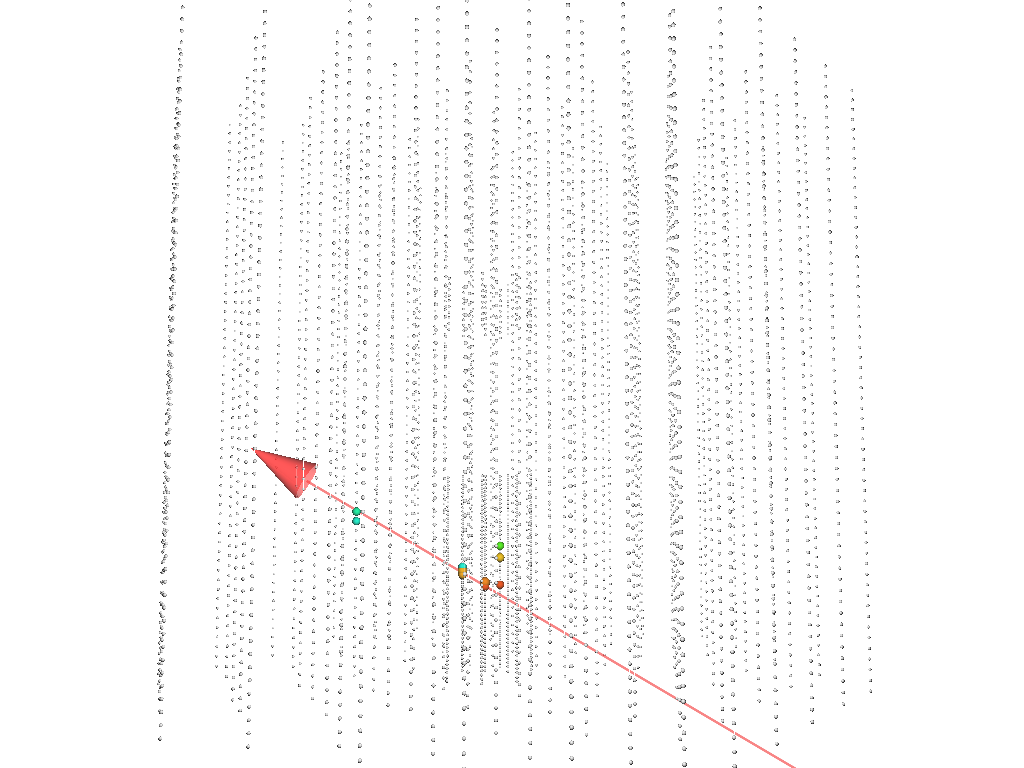
\includegraphics[width=0.49\textwidth]{appendix/img/FINAL_signal_m_100_ch1ovr3.png}
\caption{\textit{Left: }Typical simulated SMP of 100 GeV and charge 1/2 that survives the final selection. \textit{Right: }Typical simulated SMP of 100 GeV and charge 1/3 that survives the final selection. Note that there is a lot less light produced compared to particles with higher charges.}
\label{fig:final_4}
\end{figure}

\begin{figure}
\centering
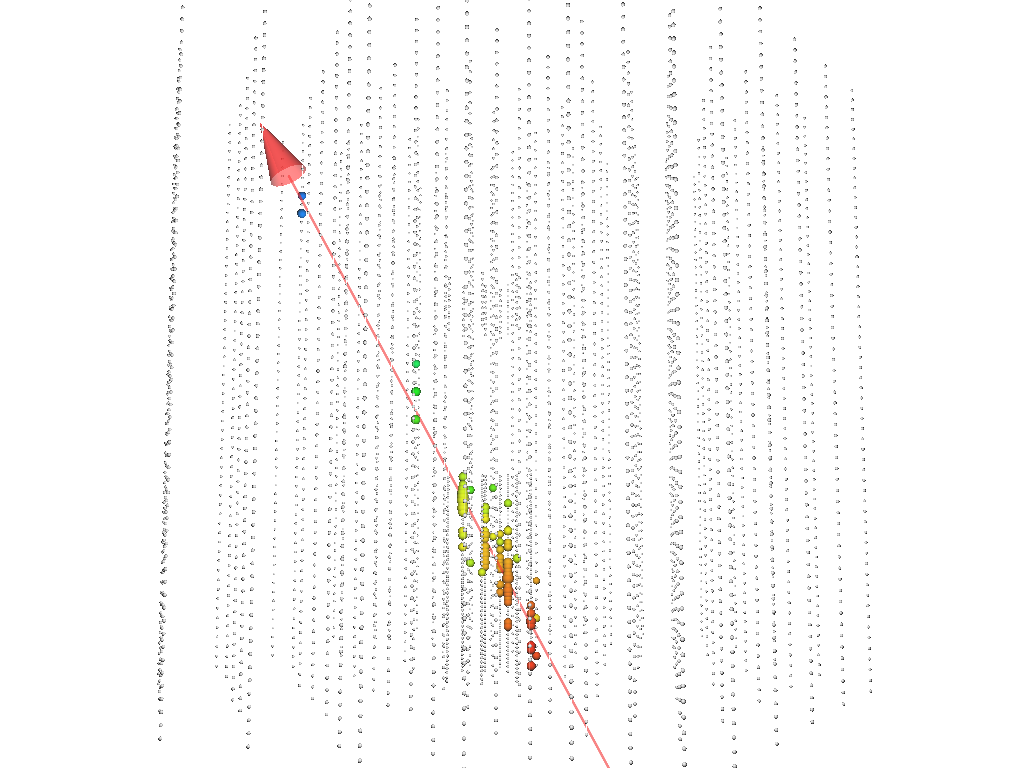
\includegraphics[width=0.49\textwidth]{appendix/img/FINAL_signal_m_100_ch2ovr3.png}
\caption{Typical simulated SMP of 100 GeV and charge 1/3 that survives the final selection. Note that there is a lot more light produced compared to particles with lower charges.}
\label{fig:final_4}
\end{figure}




\end{appendices}